% Template for FMI-2011 paper; to be used with:
%          fmiconf.sty - LaTeX style file, and
%          IEEEbib.bst - IEEE bibliography style file.
% --------------------------------------------------------------------------
\documentclass{article}
\usepackage{fmiconf,amsmath,epsfig}

\usepackage{german}
\usepackage[utf8]{inputenc}
\usepackage{url}

% Example definitions.
\def\x{{\mathbf x}}
\def\L{{\cal L}}

% Title.
\title{Kann eine Flugdrohne präzise nur mit den Sensoren eines Smartphones gesteuert werden?}
\name{Stefan Baumann, Florian Gümbel}
\address{Technische Hochschule Mittelhessen}

\begin{document}
\maketitle
\begin{abstract}
Drohne ist mittlerweile auch im Konsumbereich ein fest etablierter Begriff, der ein von vier Propellern und Elektromotor angetriebenes Flugobjekt beschreibt. Die Steuerung erfolgt zumeist über eine Anwendung auf Smartphone / Tablet. Dabei wird hauptsächlich ein virtueller Joystick auf dem Bildschirm angezeigt der mit Gesten gesteuert wird.\\ Eine andere aber bisher aber weitestgehend eingeschränkt genutzte Art der Steuerung ist der Einsatz von Hilfe Gyroscope und Accelerometer des Smartphones. Eingeschränkt insofern, als dass nicht alle Möglichkeiten der Sensoren genutzt werden. An diesem Ansatz soll mit der Entwicklung einer nativen Android App für Smartphones angeknüpft werden. Ziel ist es, die Bewegungen, die vom Benutzer mit dem Smartphone getätigt werden, an die Drohne zu übertragen. Zusätzlich sollen Gesten das Steuern von Foto- und Videoaufnahmen und deren Übertragung auf das Display des Smartphones vervollständigen.\\ Am Ende gilt es die Frage zu beantworten, ob die Steuerung einer Drohne präzise genug ist, wenn diese komplett über Gyroscope und Accelerometer des Smartphones erfolgt.

\end{abstract}

\section{Einleitung}
\label{sec:einleitung}
Immer mehr erfreuen sich sogenannte Drohnen im Konsumbereich an Beliebtheit. Diese neue Form des unbemannten Flugobjekte zeichnet sich zumeist dadurch aus, dass sie, anders als herkömmliche bekannte Modellflugzeuge, mindestens vier kleine Propeller hat welche über Elektromotoren angetrieben werden und die Drohne senkrecht starten lassen. Die Anzahl der Propeller kann variieren. Angefangen von Quadrocopter über Hexacopter und Octacopter bis hin zu Multicopter. Der Einsatzzweck einer solchen Drohne geht von Vermessungstechnik über Luftaufnahmen und Erkundung bis hin zur Jagd. In diesem Fall geht es jedoch um die für die im Privatgebrauch übliche Hobby-Flugdrohne.

Um eine Solche Drohne zu Steuern gibt es verschiedene Möglichkeiten. Abhängig von Modell lassen sich klassische Fernsteuerungen\cite{flypad} entweder direkt mit der Drohne Verbinden oder über Umweg mit Hilfe einer App. Nahezu jeder Drohnenhersteller bietet eine eigene App für alle gängigen Smartphones oder Tablets an. Die Verbindung findet je nach Modell über W-Lan oder Bluetooth statt. Für die Steuerung mittels App auf dem Gerät stehen in der bekanntesten Variante meist zwei digitale Joysticks zur Verfügung deren Bewegung umgerechnet und auf die Drohne Übertragen wird während das Gerät ruhig in der Hand liegt. Meistens ist über den linken Joystick die Veränderung der Höhe und eine Drehung möglich. Der Rechte Joystick ist für die horizontale Bewegung zuständig. Damit ist das Schwenken zur Seite sowie das Vorwärts- und Rückwärtsfliegen gemeint. Eine schwerere Variante der Steuerung ist die Richtungsangabe mittels Neigung des Gerätes.
\\ Die Idee ist es nun, eine Erweiterung der schweren Variante zu untersuchen, bei der zwei Sensoren des Smartphones zum Einsatz kommen. Dabei soll komplett auf die Bedienung von Touchscreen verzichtet und nur das Gerät selbst als Steuerungseinheit verwendet werden. Dazu dienen die beiden Sensoren (Gyroskop und Accelerometer) zur Erfassung der Bewegungen woraufhin das Smartphone diese umrechnet und auf die Drohne überträgt. 

\section{Stand der Technik}
\label{sec:verwandteArbeiten}
\subsection{Drohnensteuerung}
Neben einigen wenigen Drittherstelleranwendungen bieten, wie bereits in der Einleitung erwähnt, auch die Hersteller der Drohnen eigene Anwendungen zum steuern der Drohne an.
\\ Die bekannte Firma Parrot stellt eine Vielzahl verschiedener Apps zum Steuern bereit. Eine davon ist die FreeFlight-App \cite{freeflightapp}, die Steuerung durch den Gyroscope-Sensor unterstützt. Insgesamt bietet sie drei Möglichkeiten an wobei der Linke Joystick immer für die Höhe und Drehung zuständig ist:
\begin{description}
\item Normal \\
Wie in Abbildung \ref{fig:freeflight} gezeigt, wird auf den rechten Joystick ein Symbol angezeigt auf das dauerhaft gedrückt werden muss um die Flugrichtung der Drohne mit Neigung des Smartphone anzugeben.  
\item Ass (Experte) \\ 
Auf dem Rechten Joystick kann eine schnelle Kursänderung mittels Swipe-Geste angegeben werden während durch drücken des linken Joysticks und neigen des Smartphone eine Änderung der Flugrichtung erzielt werden kann. 
\item Joypad\\
Hierbei handelt es sich um die standardmäßige Steuerung der Drohne mittels Bewegen der beiden Joysticks
\end{description}

Bei Normal und Ass fliegt die Drohne in die Richtung in der das Smartphone geneigt wird ohne sich dabei in diese zu drehen. Eine Höhenveränderung oder Drehen durch Bewegung ist in keiner Variante möglich. Auf eine Implementierung des Accelerometer wurde hierbei verzichtet.

\begin{figure}[htb]
\begin{minipage}[b]{1.0\linewidth}
  \centering
\centerline{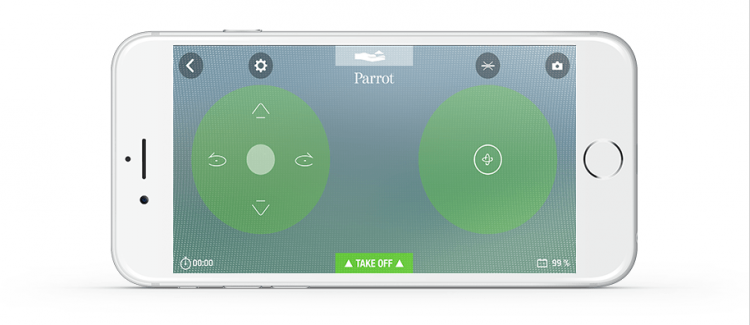
\includegraphics[width= 85mm]{freeflight_mini.png}}
\end{minipage}
\caption{Normale Steuerung (Quelle: Parrot)}
\label{fig:freeflight}
\end{figure}

Bereits Anfang 2015 hat Sony ein Projekt vorgestellt, in dem eine Drohne mittels SmartWatch 2, SmartEyeglass und Smartphone gesteuert wird \cite{sonyflight}. In diesem Fall ist die SmartWatch via Bluetooth mit dem Smartphone verbunden und überträgt die Bewegung per W-Lan an die Drohne. Über das Display der Smartwatch lassen sich dabei die verschiedenen Steuerungs-Modi umschalten. Hier kommen sowohl Accelerometer als auch Gyroscope zum Einsatz.

\subsection{Einsatz von Sensoren}
Die in Abbildung \ref{fig:gyro} gezeigten Sensoren finden in vielen Bereichen Verwendung und sind bereits in jedem aktuellen Smartphone standardmäßig verbaut. 
Sie werden meistens in Kombination genutzt wie beispielsweise bei der Erkennung von Bewegungsänderung oder der Messung von physischen Aktivitäten \cite{wu2012classification}. Aber auch bei Spielen sind sie ein gern genutztes Hilfsmittel um in Rennspielen das Lenken eines Fahrzeuges zu simulieren oder einen Balanceakt zu meistern. 
Um die derzeitige Lage oder Beschleunigung des Gerätes zu ermitteln, kommt der Accelerometer oder auch Beschleunigungssensor zum Einsatz. Mittels der Schwerkraft wird ermittelt in welche Richtung das Smartphone bewegt wird. In der Regel kommen die X- Y- und Z-Achse zum Einsatz. Die rotatorische Geschwindigkeit und somit auch die Drehbewegung des Smartphones werden vom Gyroskop gemessen. Dazu wird die Corioliskraft und das sogenannte Stimmgabelprinzip genutzt. Hier kommen Längs- Quer und Hochachse für die Positionsbestimmung im Raum zum Einsatz.

\begin{figure}
\begin{minipage}[b]{1.0\linewidth}
  \centering
\centerline{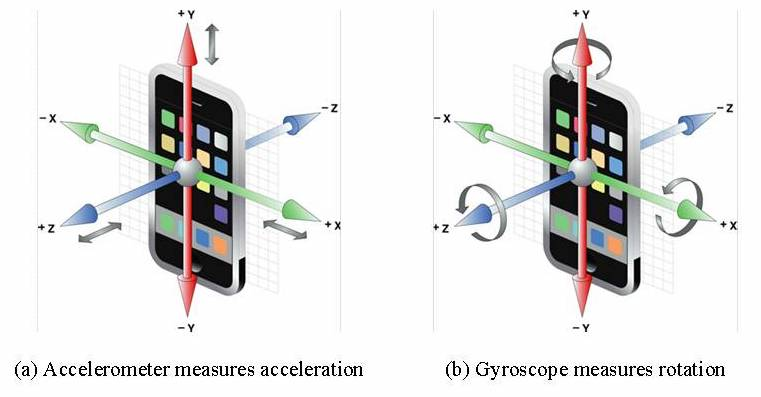
\includegraphics[width= 85mm]{gyro.jpg}}
\end{minipage}
\caption{Accelerometer und Gyroscope (Quelle: Apple Inc.)}
\label{fig:gyro}
\end{figure}

\section{Methodik}

\subsection{Eingesetzte Drohne}
Als Testdrohne wurde für eine Parrot Airborne Night Drone der Kategorie Mini-Drohne entschieden \cite{minidrone}, da sie folgende Vorteile mit sich bringt: 
\begin{itemize}
	\item Relativ geringen Anschaffungspreis
	\item Unterstützung des aktuellen Parrot SDK3
	\item Gute Testbarkeit in Gebäuden durch geringe Größe 
\end{itemize}

Des weiteren verfügt die Drohne über zwei LED- Suchscheinwerfer, einen 1GB Flashspeicher für Fotos mit der eingebauten VGA(480x640) Mini-Kamera, einen Ultraschall-Reichweitenmesser sowie ein 3-Achsen-Gyroscope und einen 3-Achsen- Beschleunigungsmesser (+\/- 50mg).

Nach einer Flugzeit von maximal 9 Minuten (ohne Schutz) kann der 550 mAh-Akku mittels Quickcharging in 25 aufgeladen werden. 

\subsection{Verwendete Technologien}
Wie in den vorangegangenen Kapitel schon erläutert wurde, gibt es aktuell keine App die eine komplette Steuerung über die Sensoren unterstützt. Aus diesen Gründen wurde zu Testzwecken ein Prototyp entwickelt, welcher die gestellten Anforderungen erfüllt. Aus Gründen der Flexibilität wurde für die Umsetzung des Prototypen für eine native Android-Anwendung zusammen mit dem SDK3 von Parrot entschieden. Die Mindestanforderung für Android ist Version 4.3.\\ 

Als Verbindung zwischen Anwendung und Drohne kommt Drohnenbedingt Bluetooth in der Version 4.0 zum Einsatz. Während größere Drohnen W-Lan anbieten, beschränkt sich die Minidronen-Reihe auf Bluetooth. Dieses ist auf 20 meter begrenzt, was angesichts der kleinen Größe und der Nutzung in Gebäuden kein Nachteil ist. 

\subsection{Zielgruppenbestimmung}
Eine Einschränkung der Zielgruppe ergibt sich aus der Entwicklung des Prototyp für die Parrot Airborne Night - Reihe oder andere Parrot Flugdrohnen die mittels Bluetooth verbunden werden. Zusätzlich ist die Nutzung auf Android fähige Smartphone in der Version 4.3 oder höher beschränkt.
  
\subsection{Vorgesehene Steuerung}
Die sinnvolle Erweiterung der bereits bestehen Steuerung ist die Kernaufgabe des Prototyp. Mit einer guten Umsetzung kann ein präzises Steuern nur mit Sensoren möglich sein. Wie bereits in der Stand der Technik beschrieben, haben beide Sensoren verschiedene Eigenschaften die sie liefern. Diese gilt es nun so einzusetzen, dass eine Steuerung durch Bewegungen so einfach wie möglich ist. Grundsätzlich gibt es an der bisher von Parrot zur Verfügung gestellten Form der Steuerung durch Bewegung nichts zu kritisieren. Sie ist vom Prinzip her logisch aufgebaut so dass der Benutzer sie Intuitive bedienen kann ohne vorher eine Betriebsanleitung lesen zu müssen. 

Daraus ergibt sich, dass zwei der drei Achsen des Gyroscopes schon in Verwendung sind. Nimmt man die Verteilung der in Abbildung \ref{fig:gyro} gezeigten Sensoren an, so ist die X-Achse bereits für die seitliche und die Y-Achse für die vor und zurück Bewegung der Drohne zuständig. Als erste Neuerung soll die Z-Achse genutzt werden um die Drehungsfunktion des linken Joysticks zu implementieren. 

Eine weitere Funktion des linken Joysticks ist die Änderung der Höhe. Hierfür eignet sich besondern die in Abbildung \ref{fig:gyro} gezeigte Z-Achse des Accelerometer. Ebenfalls kann durch eine schnelle Auf-Bewegung die Drohne starten und durch eine schnelle Abwärts-Bewegung landen. Aber auch die Swipe-Funktionen aus der Experten Variante sollen mittels Accelerometer umgesetzte werden. Die 90 Grad Drehung kann durch eine rasche Bewegung in die jeweilige Richtung ausgelöst werden. Eine schnelle Bewegung nach vorne sorgt für eine 180 Grad-Drehung über die linke Seite und eine schnelle Bewegung nach hinten für eine über die rechte Seite. 

Abbildung \ref{fig:gameplay} zeigt grafisch wie die Steuerung mit Sensoren aussehen soll. 

\begin{figure}
\begin{minipage}[b]{1.0\linewidth}
  \centering
\centerline{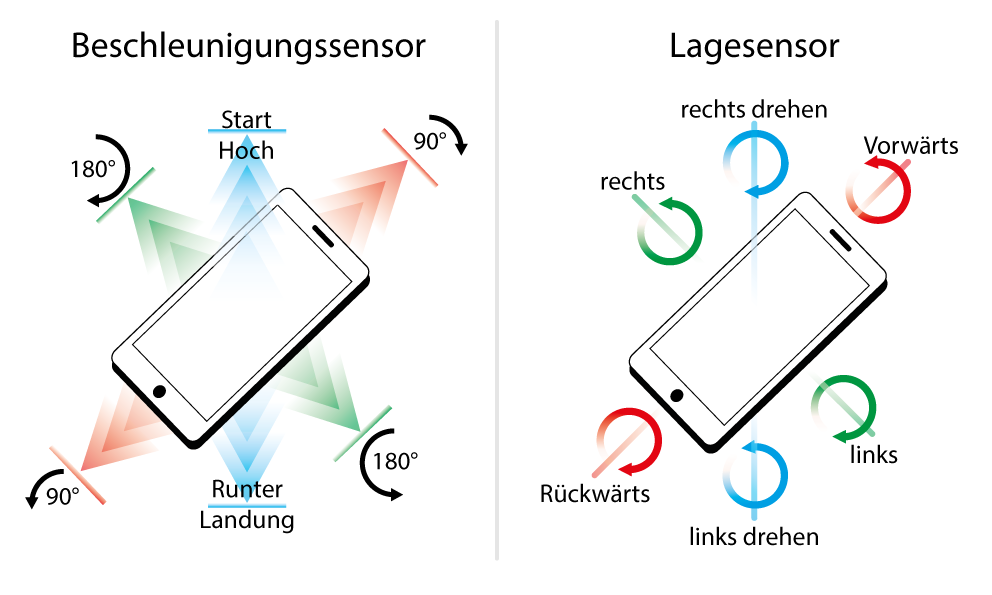
\includegraphics[width= 85mm]{gameplay}}
\end{minipage}
\caption{Steuerung mit Sensoren}
\label{fig:gameplay}
\end{figure}


Streng genommen könnte auch das auslösen der Kamera oder das Einschalten der LED zur Steuerung gehören. Da es sich bei den Tests aber um das reine Fliegen handelt, werden diese bei dem Prototyp nicht berücksichtigt.

\subsection{Umsetzung des Prototypen} 
Alle die im Kapitel Steuerung geforderten Steuerung galt es im Prototypen umzusetzen. 

\section{Ergebnisse und Evaluation}
Um die eingangs gestellte Frage ehrlich beantworten zu können muss eine Evaluation durchgeführt werden in der eine möglichst breite Maße an verschiedenen Personen den Prototyp unter gleichen Bedingungen Testet. Hierfür wurde ein Parkour aufgebaut welcher einmal mit den von Parrot gelieferten Steuerungsmöglichkeiten und einmal mit dem entwickelten Prototyp getestet werden muss. Der Parkour ist so aufgebaut, dass alle Funktionen mindestens einmal dran kommen. 
Die Alterspanne der 7 Probanden lag im Bereich von 11 bis 65 Jahren. Es wurden bewusste Tester ausgesucht die keinerlei Vorkenntnisse mit dem Fliegen einer Drohne haben. 
Zur Einführung wurden ihnen die jeweiligen Steuerungsarten erklärt. Aus Gründen der Fairness wurde auf vorherige Testflüge verzichtet.
%TODO bessere idee?
Als Ausgangslage wird die Drohne in einem Abstand von 1 meter vor die Testperson aus den Boden gestellt. Diese muss die Drohne starten und bis auf Augenhöhe in die Luft steigen lassen. Nachdem eine 180 Gras Drehung vollzogen wurde, muss die Drohne in einem Abstand von circa 1 meter um die Person herum navigiert werden. Befindet sie sich in Augenhöhe auf der gegenüberliegenden Seite der Position kann sie, nachdem sie zwei mal 90 Grad gedreht wurde, gelandet werden.
Anschließend werden die Meinungen der Testpersonen zusammen mit den Beobachtung ausgewertet werden. Diese wurden gebeten ihr persönliches empfinden zu schildern mit welcher Steuerung sie Besser zurecht kamen und mit welcher sie meinen präzise Steuern zu können.
%TODO Auswertung
Das Ergebnis ......
\section{Zusammenfassung und Ausblick}
Nach der Auswertung der Evaluation 
\bibliography{Template}{}
\bibliographystyle{IEEEbib}
\end{document}